\chapter[Gerenciamento de requisitos]{Gerenciamento de requisitos}
\section{Atributos de um requisito}
Os atributos contém as informações mais importantes daquele requisito, são suas propriedades, e é a partir dessas propriedades que se tem informações como: data de criação, origem, importância, dentre outras. Demandam atenção durante a sua especificação, pois fornecem importantes informações sobre o estado do projeto, além de permitirem que sejam realizadas consultas dentro de todos os requisitos.
Os atributos definidos para gerenciar os requisitos durante a execução do nosso projeto foram:
  \begin{figure}[!htbp]
    \centering
    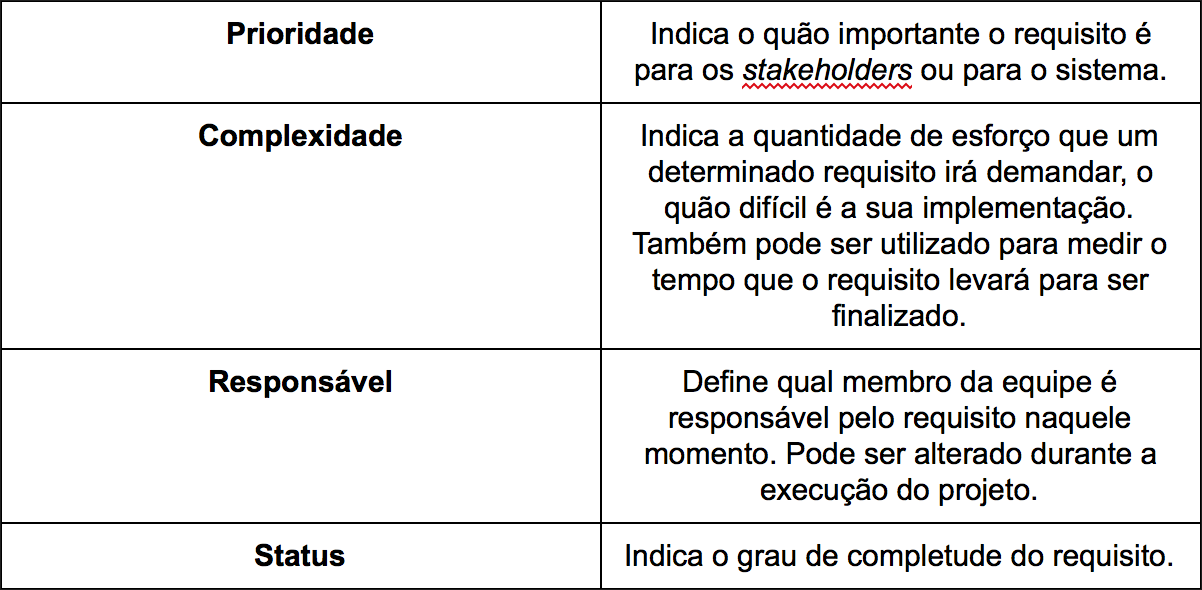
\includegraphics[scale=0.65]{editaveis/figuras/tabela_atributos}
    \caption[Atributos dos requisitos do projeto]{Atributos dos requisitos do projeto. \footnotemark}
    \label{tabela_atributos}
  \end{figure}
  
  Exemplo de matriz de atributos de requisitos:
    \begin{figure}[!htbp]
    \centering
    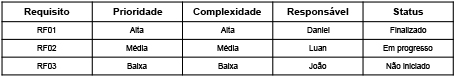
\includegraphics[scale=0.65]{editaveis/figuras/matriz_atributos}
    \caption[Matriz de atributos do projeto.]{Matriz de atributos do projeto. \footnotemark}
    \label{tabela_matriz_atributos}
  \end{figure}
\subsection{Prioridade}
  \begin{figure}[!htbp]
    \centering
    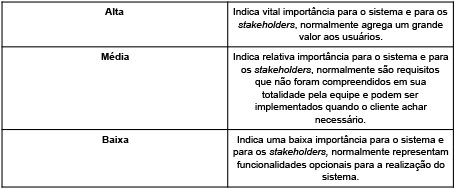
\includegraphics[scale=0.5]{editaveis/figuras/tabela_prioridade}
    \caption[Prioridade dos requisitos do projeto.]{Prioridade dos requisitos do projeto. \footnotemark}
    \label{tabela_prioridade}
  \end{figure}
\subsection{Complexidade}
  \begin{figure}[!htbp]
    \centering
    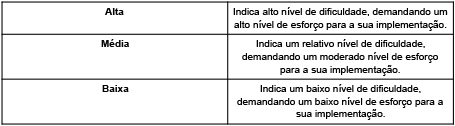
\includegraphics[scale=0.5]{editaveis/figuras/tabela_complexidade}
    \caption[Complexidade dos requisitos do projeto.]{Complexidade dos requisitos do projeto. \footnotemark}
    \label{tabela_complexidade}
  \end{figure}
\subsection{Responsável}
Identifica na equipe o membro responsável pelo requisito naquele momento.
\subsection{Status}
  \begin{figure}[!htbp]
    \centering
    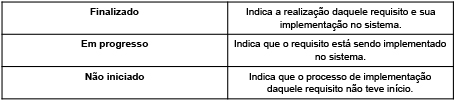
\includegraphics[scale=0.5]{editaveis/figuras/tabela_status}
    \caption[Status dos requisitos do projeto.]{Status dos requisitos do projeto. \footnotemark}
    \label{tabela_status}
  \end{figure}
\section{Rastreabilidade de requisitos}
Rastreabilidade de software é a habilidade de relacionar artefatos criados durante o ciclo de vida de desenvolvimento de um sistema de software.[1] Os elementos rastreáveis do projeto são chamados de itens de rastreabilidade.
O rastreamento de requisitos pode ser visto como uma habilidade de acompanhar e descrever a vida de um requisito em abas as direções. A pré-rastreabilidade documenta o contexto a partir do qual emergem os requisitos, já a pós-rastreabilidade vincula os requisitos ao desenho do sistema e sua implementação.(DAVIS, 1993).
(FINALIZAR)
\section{Gestão de requisitos}